\documentclass[main.tex]{subfiles}

\begin{document}

\section{Model}

\begin{figure}
  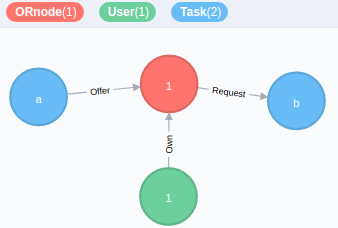
\includegraphics[]{example1.png}
  \caption{User 1 uploads an ORpair to offer task a and requests task b in exchange.}
  \label{example1}
\end{figure}

\begin{figure}
  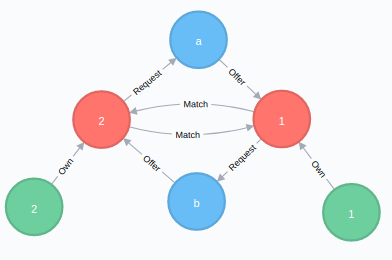
\includegraphics[]{example2.png}
  \caption{User 2 uploads an ORpair to offer task b and requests task a in exchange.
           \\Now there is a cycle/match.}
  \label{example2}
\end{figure}

An \textbf{offer network} instance can be formally modeled as a directed graph, $G$, where vertices $task \in T$ represent tasks, $user \in U$ users, and labeled directed edges $(task_a,task_b)$ represent an offer by user $user_1$ to do task $task_a$ in exchange requested task $task_b$. Due to implemention details in Neo4j\footnote{\url{https://neo4j.com/}}, (offer, request) nodes are created for labeled directed edges, called \textbf{ORpairs}. This is the \textbf{the task-centric model}\footnote{An alternative is an \textbf{ORpair-centric model} where each ORpair is directly linked to all offer or request compatible ORpairs.}.  See Figure \ref{example1}.

A matching of users who can satisfy each other is a vertex cycle. See the simplest case below in Figure \ref{example2}. There is a match acceptance probability $p$, which is assumed to be uniform and independent\footnote{Moreover, Dickerson \cite{Dick} notes this assumption potentially also protect users, such as badly sick patients, from being marginalized in addition to being simpler to analyze.}.

\subsection{Scale-Free Task Distribution}
The ReadItSwapIt data is scale-free. This means that for large degrees $k$, the fraction of nodes with degree k is proportional to $k^{-\gamma}$\footnote{\url{https://en.wikipedia.org/wiki/Scale-free_network}}. $\gamma$ is called the power law exponent. Abbassi \cite{Abb2} do not provide much anlaytics of the ReadItSwapIt data; however they experiment with $\gamma = \{0,0.25,0.5,0.75,1\}$. In colloquial terms, this means that a few tasks are very popular and most tasks are only offered or requested by a few users. There will likely be a small difference in \textit{offer} and \textit{request} popularity for tasks.

Worth mentioning on this note is a user-centric study of the eBay graph \cite{ebay}\footnote{The data is obtained via crawling eBay feedback.}. They noted the following properties on eBay:

\begin{itemize}
  \item Skewed degree distribution: i.e., there are a few big sellers.
  \item Dissasortativity: users tend to buy and sell different types of products.
  \item Linear preferential attachment in terms of positive feedback.
     \\ Strong aversion avoidance of users with negative feedback.
  \item Densification over time.
  \item No rich club connectivity (basically because big nodes are mass sellers).
\end{itemize}

Dissasortativity implies that there will be little clustering: there will be many ORpairs between diverse task types\footnote{The specialization of many exchange sites and services may seem to contradict this; however this may also be due to the ease of developing specialized mechanisms.}.

Densification over time implies new ORpairs are added at a faster rate than new tasks.

\subsubsection{Scale-Free Graph Model}
The goal is to generate a graph with a power law distribution with a small difference in the in and out degree distributions. To this end a generator for directed scale-free graphs is modified. The modified graph generator from NetworkX \cite{netX} is described by Bollobás, Borgs, Chayes, and Riordan in \textit{Directed Scale-Free Graphs} \cite{Bol}. It's a preferential attachment model.

The graph starts with a directed triangle.

Each time an edge\footnote{ORpair} is added with probability $p_d$ the directed scale-free graph generation is used that chooses nodes based on in/out-degree, otherwise node choice is based on total degree.
\begin{itemize}
  \item $\alpha$, create new node\footnote{task} $v$ and choose $w$ based on in-degree distribution.
  \item $\gamma$, create new node $w$ and choose $v$ based on out\_degree distribution.
  \item $\beta$, choose $v$ based on out-degree distribution and $w$ based on in-degree distribution.
\end{itemize}
Then add $(v,w)$ to the graph.

There are parameters $\delta_{in}$ and $\delta_{out}$ added to the degree so that nodes with zero degree are still chosen with non-zero probability (and $\frac{\delta_{in} + \delta_{out}}{2}$ in the total degree case). Let
$$c_1 = \frac{\alpha + \beta}{1 + \delta_{in}(\alpha + \gamma)} \mbox{ and } c_2 = \frac{\beta + \gamma}{1 + \delta_{out}(\alpha + \gamma)}$$
$$X_{IN} = 1 + 1/c_1 + c_2/c_1(\delta_{out} + 1_{\{\gamma \delta_{out}=0\}})$$
$$X_{OUT} = 1 + 1/c_2 + c_1/c_2(\delta_{in} + 1_{\{\alpha \delta_{out}=0\}})$$
$X_{IN}$ and $X_{OUT}$ are the power law exponents. Note that in this model in-degree and out-degree distributions are independent. The non-directed power law exponent is ???.

The modification of the model generates a set number of edges and for each edge adds a new task with probability $\alpha + \gamma$.

\subsection{Dynamics}
The dynamic offer network experiment starts with a scale free graph generated as above with $N^o_{initial}$ ORpairs. Each step 1 ORpair is added. There are $n^u$ ORpairs for each user, so every $n^u$ steps a user is added. With probability $\alpha + \gamma$ a new task is added with the ORpair. The experiment is run until $N^o_{end}$ ORpairs have been added. Every $n_{match}$ steps matchings are suggested, accepted or rejected by users, and accepted ORpairs are removed from the graph.

It is possible to make $n^u$ be probabilistic as with new tasks, and it's possible to make $n_{match}$ depend on the graph size.

The series of graph updates from the start to completion $N_{end}^o$ are pre-generated so that all algorithms can be tested on the same dynamic graph. Note that the graph used to determine the scale-free task distribution (in NetworkX) is separate from the offer network graph (in Neo4k) that the matching is done on. This is to prevent ORpairs being matchend and removed from altering the task distribution\footnote{In reality, there will be a relation between these; however, modeling this relation is beyond the scope of the thesis. Futhermore, more matches of a certain task are likely to increase the task popularity.}

\subsection{Cycle Size and Acceptance Probability}

\subsubsection{Motivation}
The optimal solution clearly depends on acceptance probability, primarily biased by the optimal cycle size. In general, finding a maximum edge-disjoint cycle cover with cycle-weights (to account for acceptance probability) is NP-hard \cite{Bir}. Dickerson \cite{Dick} \cite{Dick3} find that integer linear programming with a model that optimizes for expected gain based on a uniform or bi-modal (high and low) acceptance probability performs linearly better\footnote{$A$ performs linearly better than $B$ means $Utility(A,n) = Utility(B,n) + \Omega(n)$.}.

When using heuristics, however, one possibility is to simply choose a different algorithm depending on the currest estimation for $p$. Included below is some basic probabilistic guidance.

\subsubsection{Analysis}

\begin{figure}
  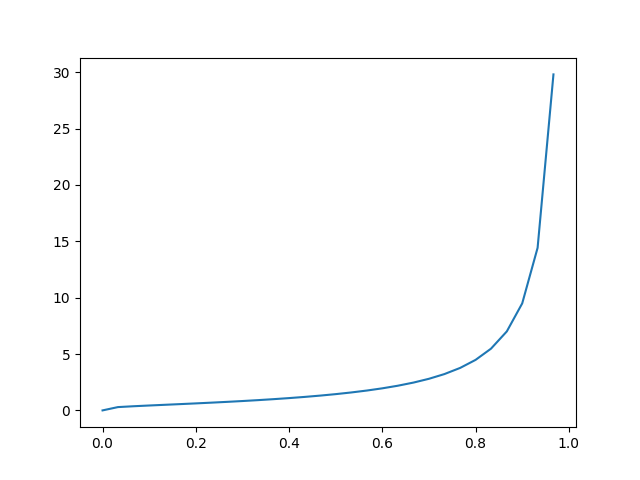
\includegraphics[scale=0.65]{best-k.png}
  \caption{Best k-cycle for p from 0.8 to 1}
  \label{best-k}
\end{figure}

\begin{figure}
  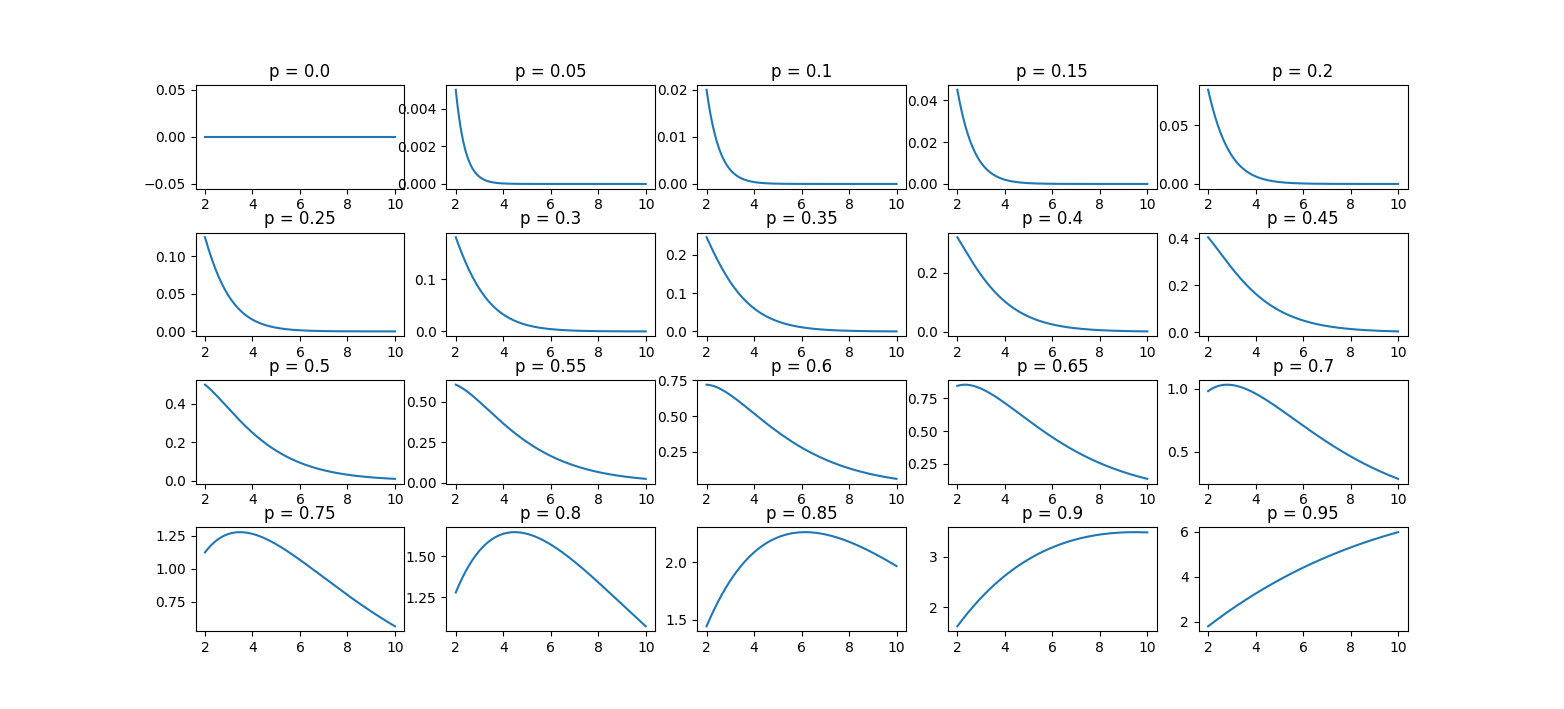
\includegraphics[width=\textwidth]{eckp1.png}
  \caption{$\E[c_k]$ for $k = 2 \dots 10$}
  \label{eckp1}
\end{figure}

\begin{figure}
  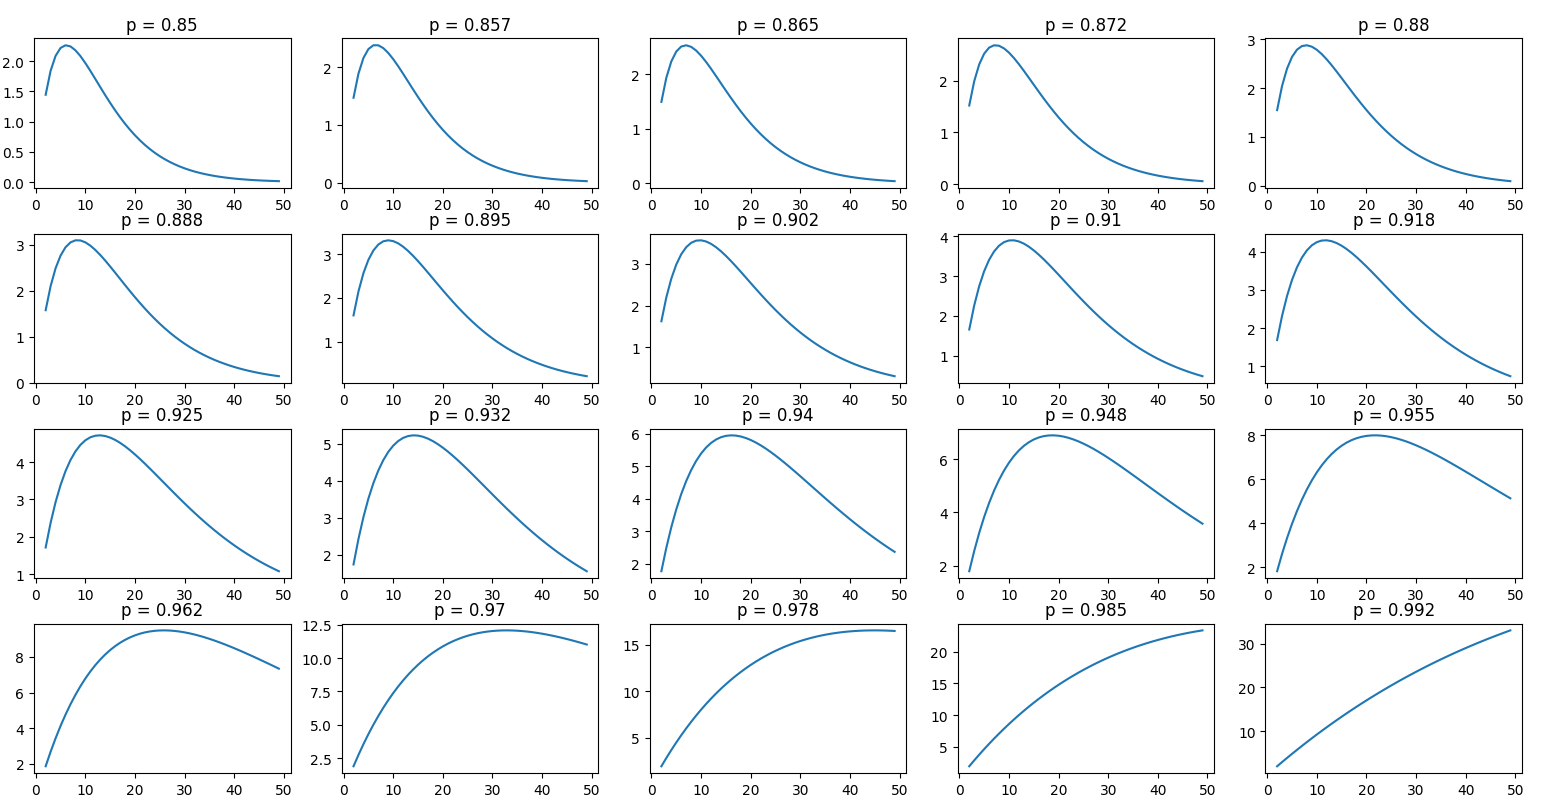
\includegraphics[width=\textwidth]{eckp2.png}
  \caption{$\E[c_k]$ for $k = 2 \dots 50$}
  \label{eckp2}
\end{figure}

In a cycle $c$ of size $k$, the probability of acceptance is $p_k = p^k$.

Thus the expected number of satisfied users is: $\E[c_k] = k p^k$. For a given $p$, the best cycle size is given by $k = -\frac{1}{\ln p}$, and the best attainable for $p$ is $-\frac{1}{e \ln p}$.

As can be seen in Figure \ref{best-k}, the optimal cycle size exponentially incresaes above $p = 0.95$ ($k \approx 19$), so the maximum without cycle-length constraints will likely suffice\footnote{Unless the algorithm retruns 1000+ length cycles.}. And in Figures \ref{eckp1} \ref{eckp2} one sees that $2$-cycles are optimal for low-p, $p < 0.7$. The PTIME heuristic is less clear for the following cases:
\begin{itemize}
  \item mid-p: $0.7 < p < 0.85$ where $ 2 < k < 10$ is optimal.
  \item high-p: $0.85 < p < 0.95$ where $ 10 < k < 30$ is optimal,
      \\yet the larger cycles are little bitter than shorter ones.
\end{itemize}

For human users without very specific task formulations, $p$ likely lies in this range. However, Dickerson \cite{Dick} \cite{Dick3} found that with kidney exchanges, $p < 0.3$.

\subsubsection{How many matches are needed to for acceptance?}\label{sec:nrounds}
This thesis tests a heuristic to make long-cycles feasible even without high $p$. The heuristic satisfies an ORpair if both of its neighbors in the cycle also accept the suggested match (rather than if all users in the cycle accept). If one of the neighbors does not accept the match, then the user is rematched in a way explained in the Methods seciton. The feasibility of this approach depends on how many times a user can expect to be rematched.

In a given round, the probability the suggested match goes through is $p^3$ as both neighbors in a cycle also need to accept. Thus the expected number of rounds for acceptance follows the geometric distribution: $\sum_{k=0}^{\infty} k p^3 (1 - p^3)^{k-1} = \frac{1}{p^3}$.

\begin{figure}
  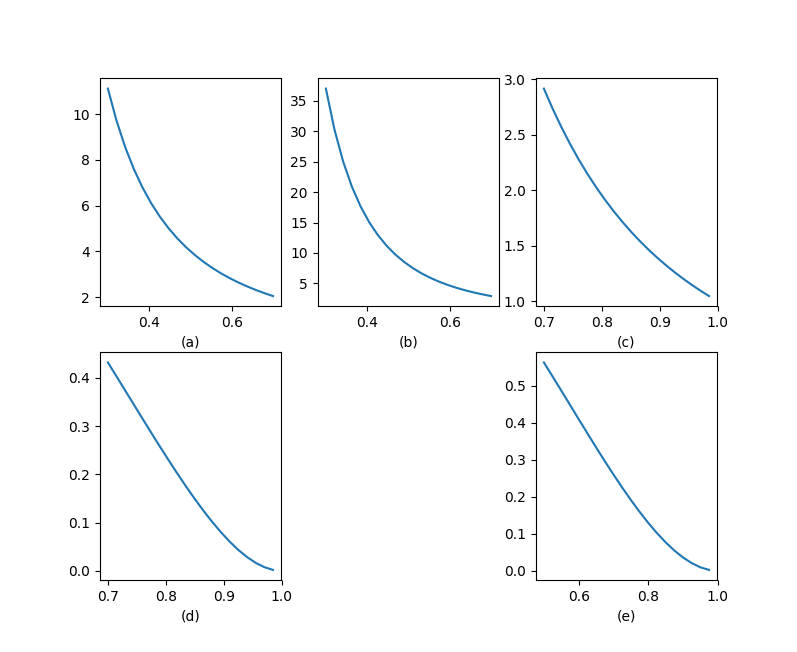
\includegraphics[width=\textwidth]{nrounds.png}
  \caption{(a)-(c) plot expected number of rounds for acceptance of an ORpair for different $p$. (a) is for 2-cyles. (b) and (c) for k-cycles. (d) and (e) plot the probability of an ORpair not being accepted in 2 rounds. (d) is for k-cycles and (e) is for 2-cycles.}
  \label{nrounds}
\end{figure}

As one can see in Figure \ref{nrounds}, one expects 5 rounds to be needed by $p = 0.6$. Fortunately, for $p > 0.7$, one expcets less than 3 rounds to be needed. With 2-cycles, one only needs 3 or 4 rounds for $p = 0.6$ or $0.5$. For lower $p$, the offer network may become frustrating for human users: something will have to be done to increase acceptance probability. For example, matching may have to be done on more detailed task specifications \footnote{Acceptance probaility is likely proportional to how detailed task specifications are; however, there are also limits as to how detailed humans can be. The reasoning is that when a user rejects a match it is probably because of an unspecified criteria not met. An example in the kidney case is crossmatch testing: $70\%$ of post-match rejections are because of positive crossmatch that is expensive to test. Dickerson \cite{Dick} find that even a random sapmle of crossmatch tests, that is more detailed specifications, allow for many more matches.}.

One can also easily calculate the probability acceptance for an ORpair will take more than two rounds: $1 - (p^3 + p^3 * (1 - p^3))$.

\subsubsection{Application to Kidney Exchange}
When exchanging kidneys there is a type of incompatibility not checked prior to initial matching: PRA (percent reactive antibody). Roth et al. \cite{Rot2} split the distribution into low, medium, and high PRA with respective 5, 45, and 90 percent probability of positive crossmatch (rejection). The frequency among kidney donors is 70, 20, and 10 percent. Thus for 10 percent of matches, anything but 2-cycle has very low expectation, and for another 20 percent, 2-cycle is still expected to perform twice as well as 4-cycle matches. For the remaining 70 percent, however, 20-cycle matches are best, and 50-cycle still preferable to anything less than 10-cycle matches.

Thus when mixing low, medium, and high PRA the result that 4-cycle matches don't help much makes sense \cite{Rot2}.

Morevore, Dickerson \cite{Dick} \cite{Dick3} calculates acceptance probabiltiy\footnote{Optimistically based on only positive crossmatch.} to be at most $30$ percent: that is, 2-cycle matches are always preferable to 3-cycle.

\end{document}


%% For loading example graph into Neo4j
%%CREATE (t1:Task {id:'a'})
% CREATE (t2:Task {id:'b'})
% CREATE (u:User {id:'1'})
% CREATE (u2:User {id:'2'})
% CREATE (o:ORpair {id:'1', offer:'a', request:'b', user:'1'})
% CREATE (o2:ORpair {id:'2', offer:'b', request:'a', user:'2'})
% CREATE (t1)-[:Offer]->(o)-[:Request]->(t2)
% CREATE (t2)-[:Offer]->(o2)-[:Request]->(t1)
% CREATE (u)-[:Own]->(o)
% CREATE (u2)-[:Own]->(o2)

% Replacing:
%
% \begin{center}
  % \begin{tikzpicture}
    % \node[draw, circle] (ta) at (0,0) {$t_a$};
    % \node[draw, circle] (tb) at (6,0) {$t_b$};
    % \draw[-latex] (ta) to[bend left=10] node[above] {$u_1$} (tb);
    % \draw[-latex] (tb) to[bend left=10] node[below] {$u_2$ }(ta);
  % \end{tikzpicture}
% \end{center}
%
% \begin{center}
  % \begin{tikzpicture}
    % \node[draw, circle] (ta) at (0,0) {$t_a$};
    % \node[draw, circle] (tb) at (6,0) {$t_b$};
    % \path [->] (ta) edge node[above] {$u_1$} (tb);
  % \end{tikzpicture}
